% (find-LATEX "2022-2-C3-derivadas-parciais.tex")
% (defun c () (interactive) (find-LATEXsh "lualatex -record 2022-2-C3-derivadas-parciais.tex" :end))
% (defun C () (interactive) (find-LATEXsh "lualatex 2022-2-C3-derivadas-parciais.tex" "Success!!!"))
% (defun D () (interactive) (find-pdf-page      "~/LATEX/2022-2-C3-derivadas-parciais.pdf"))
% (defun d () (interactive) (find-pdftools-page "~/LATEX/2022-2-C3-derivadas-parciais.pdf"))
% (defun e () (interactive) (find-LATEX "2022-2-C3-derivadas-parciais.tex"))
% (defun o () (interactive) (find-LATEX "2022-2-C3-derivadas-parciais.tex"))
% (defun u () (interactive) (find-latex-upload-links "2022-2-C3-derivadas-parciais"))
% (defun v () (interactive) (find-2a '(e) '(d)))
% (defun d0 () (interactive) (find-ebuffer "2022-2-C3-derivadas-parciais.pdf"))
% (defun cv () (interactive) (C) (ee-kill-this-buffer) (v) (g))
%          (code-eec-LATEX "2022-2-C3-derivadas-parciais")
% (find-pdf-page   "~/LATEX/2022-2-C3-derivadas-parciais.pdf")
% (find-sh0 "cp -v  ~/LATEX/2022-2-C3-derivadas-parciais.pdf /tmp/")
% (find-sh0 "cp -v  ~/LATEX/2022-2-C3-derivadas-parciais.pdf /tmp/pen/")
%     (find-xournalpp "/tmp/2022-2-C3-derivadas-parciais.pdf")
%   file:///home/edrx/LATEX/2022-2-C3-derivadas-parciais.pdf
%               file:///tmp/2022-2-C3-derivadas-parciais.pdf
%           file:///tmp/pen/2022-2-C3-derivadas-parciais.pdf
% http://angg.twu.net/LATEX/2022-2-C3-derivadas-parciais.pdf
% (find-LATEX "2019.mk")
% (find-sh0 "cd ~/LUA/; cp -v Pict2e1.lua Pict2e1-1.lua Piecewise1.lua ~/LATEX/")
% (find-sh0 "cd ~/LUA/; cp -v Pict2e1.lua Pict2e1-1.lua Pict3D1.lua ~/LATEX/")
% (find-sh0 "cd ~/LUA/; cp -v C2Subst1.lua C2Formulas1.lua ~/LATEX/")
% (find-CN-aula-links "2022-2-C3-derivadas-parciais" "3" "c3m222dp" "c3dp")

% «.defs»			(to "defs")
% «.title»			(to "title")
% «.links»			(to "links")
% «.um-exemplo»			(to "um-exemplo")
% «.exercicio-0»		(to "exercicio-0")
% «.encontrar-coeficientes»	(to "encontrar-coeficientes")
% «.exercicio-1»		(to "exercicio-1")
% «.o-macaco»			(to "o-macaco")
% «.exercicio-2»		(to "exercicio-2")
% «.normal-e-gradiente»		(to "normal-e-gradiente")
% «.exercicio-3»		(to "exercicio-3")
% «.exercicio-4»		(to "exercicio-4")
%
% «.djvuize»	(to "djvuize")



% <videos>
% Video (not yet):
% (find-ssr-links     "c3m222dp" "2022-2-C3-derivadas-parciais")
% (code-eevvideo      "c3m222dp" "2022-2-C3-derivadas-parciais")
% (code-eevlinksvideo "c3m222dp" "2022-2-C3-derivadas-parciais")
% (find-c3m222dpvideo "0:00")

\documentclass[oneside,12pt]{article}
\usepackage[colorlinks,citecolor=DarkRed,urlcolor=DarkRed]{hyperref} % (find-es "tex" "hyperref")
\usepackage{amsmath}
\usepackage{amsfonts}
\usepackage{amssymb}
\usepackage{pict2e}
\usepackage[x11names,svgnames]{xcolor} % (find-es "tex" "xcolor")
\usepackage{colorweb}                  % (find-es "tex" "colorweb")
%\usepackage{tikz}
%
% (find-dn6 "preamble6.lua" "preamble0")
%\usepackage{proof}   % For derivation trees ("%:" lines)
%\input diagxy        % For 2D diagrams ("%D" lines)
%\xyoption{curve}     % For the ".curve=" feature in 2D diagrams
%
\usepackage{edrx21}               % (find-LATEX "edrx21.sty")
\input edrxaccents.tex            % (find-LATEX "edrxaccents.tex")
\input edrx21chars.tex            % (find-LATEX "edrx21chars.tex")
\input edrxheadfoot.tex           % (find-LATEX "edrxheadfoot.tex")
\input edrxgac2.tex               % (find-LATEX "edrxgac2.tex")
%\usepackage{emaxima}              % (find-LATEX "emaxima.sty")
%
%\usepackage[backend=biber,
%   style=alphabetic]{biblatex}            % (find-es "tex" "biber")
%\addbibresource{catsem-slides.bib}        % (find-LATEX "catsem-slides.bib")
%
% (find-es "tex" "geometry")
\usepackage[a6paper, landscape,
            top=1.5cm, bottom=.25cm, left=1cm, right=1cm, includefoot
           ]{geometry}
%
\begin{document}

\catcode`\^^J=10
\directlua{dofile "dednat6load.lua"}  % (find-LATEX "dednat6load.lua")
%L dofile "Piecewise1.lua"           -- (find-LATEX "Piecewise1.lua")
%L dofile "QVis1.lua"                -- (find-LATEX "QVis1.lua")
%L dofile "Pict3D1.lua"              -- (find-LATEX "Pict3D1.lua")
%L dofile "C2Formulas1.lua"          -- (find-LATEX "C2Formulas1.lua")
%L Pict2e.__index.suffix = "%"
\pu
\def\pictgridstyle{\color{GrayPale}\linethickness{0.3pt}}
\def\pictaxesstyle{\linethickness{0.5pt}}
\def\pictnaxesstyle{\color{GrayPale}\linethickness{0.5pt}}
\celllower=2.5pt

% «defs»  (to ".defs")
% (find-LATEX "edrx21defs.tex" "colors")
% (find-LATEX "edrx21.sty")

\def\u#1{\par{\footnotesize \url{#1}}}

\def\drafturl{http://angg.twu.net/LATEX/2022-2-C3.pdf}
\def\drafturl{http://angg.twu.net/2022.2-C3.html}
\def\draftfooter{\tiny \href{\drafturl}{\jobname{}} \ColorBrown{\shorttoday{} \hours}}

\def\ddx{\frac{d}{dx}}
\def\ddy{\frac{d}{dy}}



%  _____ _ _   _                               
% |_   _(_) |_| | ___   _ __   __ _  __ _  ___ 
%   | | | | __| |/ _ \ | '_ \ / _` |/ _` |/ _ \
%   | | | | |_| |  __/ | |_) | (_| | (_| |  __/
%   |_| |_|\__|_|\___| | .__/ \__,_|\__, |\___|
%                      |_|          |___/      
%
% «title»  (to ".title")
% (c3m222dpp 1 "title")
% (c3m222dpa   "title")

\thispagestyle{empty}

\begin{center}

\vspace*{1.2cm}

{\bf \Large Cálculo 3 - 2022.2}

\bsk

Aulas 16 e 19: Derivadas Parciais

e Vetor Gradiente

\bsk

Eduardo Ochs - RCN/PURO/UFF

\url{http://angg.twu.net/2022.2-C3.html}

\end{center}

\newpage

% «links»  (to ".links")
% (c3m222dpp 2 "links")
% (c3m222dpa   "links")
% (c3m221tudop 2 "parts")
% (c3m221tudoa   "parts")
% (c3m212tudop 2 "parts")
% (c3m212tudoa   "parts")
% (c3m221nfp 10 "exercicios-3-e-4")
% (c3m221nfa    "exercicios-3-e-4")
% (c3m221nfp 12 "variaveis-novas")
% (c3m221nfa    "variaveis-novas")
% (c3m221nfp 13 "derivadas-parciais-th")
% (c3m221nfa    "derivadas-parciais-th")
% (c3m212nfp 21 "derivadas-parciais-th")
% (c3m212nfa    "derivadas-parciais-th")
% (c3m222ptp 5 "primeiros-pltans")
% (c3m222pta   "primeiros-pltans")

% (find-apexcalculuspage (+ 10 700) "12.3 Partial Derivatives")
% (find-apexcalculuspage (+ 10 711)      "12.3 Exercises")

% (find-books "__analysis/__analysis.el" "apex-calculus")
% (find-books "__analysis/__analysis.el" "apex-calculus" "4.4 Differentials")
% (find-books "__analysis/__analysis.el" "apex-calculus" "12.3 Partial Derivatives")
% (find-books "__analysis/__analysis.el" "apex-calculus" "12.3 Exercises")
% (find-books "__analysis/__analysis.el" "leithold")
% (find-books "__analysis/__analysis.el" "leithold" "3.1. A reta tangente e a derivada")
% (find-books "__analysis/__analysis.el" "leithold" "3.1. A reta tangente e a derivada" "at")
% (find-books "__analysis/__analysis.el" "leithold" "4.9. A diferencial")
% (find-books "__analysis/__analysis.el" "leithold"   "reescritas usando")
% (find-books "__analysis/__analysis.el" "miranda")
% (find-books "__analysis/__analysis.el" "miranda" "4.7 Aproximações Lineares e Diferencial")
% (find-books "__analysis/__analysis.el" "thomas" "14 Partial Derivatives")
% (find-books "__analysis/__analysis.el" "thomas" "14.3 Partial Derivatives")
% (find-books "__analysis/__analysis.el" "thomas" "Exercises 14.3")
% (find-books "__analysis/__analysis.el" "thompson")
% (find-books "__analysis/__analysis.el" "thompson" "IX. Introducing a Useful Dodge")
% (find-books "__analysis/__analysis.el" "thompson" "XVI. Partial Differentiation")
% (find-THfile "mathologer-calculus-easy.blogme")

% (find-LATEXgrep "grep --color=auto -niH --null -e apex 2022*.tex")

% (find-books "__analysis/__analysis.el" "marsden-weinstein")


{\bf Alguns links}

\scalebox{0.6}{\def\colwidth{14cm}\firstcol{

Na aula passada nós vimos derivadas parciais, mas sem esse nome:

{\scriptsize

% (c3m222ptp 5 "primeiros-pltans")
% (c3m222pta   "primeiros-pltans")
%    http://angg.twu.net/LATEX/2022-2-C3-plano-tangente.pdf
\url{http://angg.twu.net/LATEX/2022-2-C3-plano-tangente.pdf}

}

\msk


APEX Calculus: diferenciais (sec.4.4), derivadas parciais (sec.12.3):

{\scriptsize

% (find-books "__analysis/__analysis.el" "apex-calculus")
% (find-books "__analysis/__analysis.el" "apex-calculus" "4.4 Differentials")
%    http://angg.twu.net/2022.2-C3/APEX_Calculus_Version_4_cap_4.pdf#page=27
\url{http://angg.twu.net/2022.2-C3/APEX_Calculus_Version_4_cap_4.pdf\#page=27}

% (find-books "__analysis/__analysis.el" "apex-calculus" "12.3 Partial Derivatives")
% (find-books "__analysis/__analysis.el" "apex-calculus" "12.3 Exercises")
%    http://angg.twu.net/2022.2-C3/APEX_Calculus_Version_4_cap_12.pdf#page=23
\url{http://angg.twu.net/2022.2-C3/APEX_Calculus_Version_4_cap_12.pdf\#page=23}

}

\msk

Bortolossi: o cap.5 dele é sobre derivadas parciais:

{\scriptsize

% (find-books "__analysis/__analysis.el" "bortolossi")
% (find-books "__analysis/__analysis.el" "bortolossi" "5. Derivadas parciais")
\url{http://angg.twu.net/2019.2-C3/Bortolossi/bortolossi-cap-5.pdf}

}

\msk

O Leithold define a notação $\left. \frac{dy}{dx} \right]_{x=x_0}$ na p.145 (sec.3.1)

e a seção 4.9 dele (p.269) é sobre a diferencial.

% (find-books "__analysis/__analysis.el" "leithold")
% (find-books "__analysis/__analysis.el" "leithold" "3.1. A reta tangente e a derivada")
% (find-books "__analysis/__analysis.el" "leithold" "3.1. A reta tangente e a derivada" "at")
% (find-books "__analysis/__analysis.el" "leithold" "4.9. A diferencial")

\msk

Miranda: a seção 4.7 dele fala sobre diferenciais:

{\scriptsize

% (find-books "__analysis/__analysis.el" "miranda")
% (find-books "__analysis/__analysis.el" "miranda" "4.7 Aproximações Lineares e Diferencial")
% (find-dmirandacalcpage 65 "II Derivadas")
%    http://hostel.ufabc.edu.br/~daniel.miranda/calculo/calculo.pdf#page=117
\url{http://hostel.ufabc.edu.br/~daniel.miranda/calculo/calculo.pdf\#page=117}

}


\msk

Thomas: a seção 14.3 dele é sobre derivadas parciais:

{\scriptsize

%    http://angg.twu.net/2020.2-C3/thomas_secs_14.1_ate_14.7.pdf#page=21
\url{http://angg.twu.net/2020.2-C3/thomas_secs_14.1_ate_14.7.pdf\#page=21}

}

\msk

Silvanus Thompson:

o capítulo 9 dele é sobre o truque das variáveis dependentes novas,

e o capítulo 16 dele é sobre derivadas parciais:

{\scriptsize

%    https://calculusmadeeasy.org/9.html
\url{https://calculusmadeeasy.org/9.html}

% (find-books "__analysis/__analysis.el" "thompson" "IX. Introducing a Useful Dodge")
%    https://www.gutenberg.org/files/33283/33283-pdf.pdf#page=77
\url{https://www.gutenberg.org/files/33283/33283-pdf.pdf\#page=77}

% (c3m221nfp 12 "variaveis-novas")
% (c3m221nfa    "variaveis-novas")
%    http://angg.twu.net/LATEX/2022-1-C3-notacao-de-fisicos.pdf#page=12
\url{http://angg.twu.net/LATEX/2022-1-C3-notacao-de-fisicos.pdf\#page=12}
\standout{$←$ comece por aqui!}

\ssk

%    https://calculusmadeeasy.org/16.html
\url{https://calculusmadeeasy.org/16.html}

% (c3m221nfp 13 "derivadas-parciais-th")
% (c3m221nfa    "derivadas-parciais-th")
%    http://angg.twu.net/LATEX/2022-1-C3-notacao-de-fisicos.pdf#page=13
\url{http://angg.twu.net/LATEX/2022-1-C3-notacao-de-fisicos.pdf\#page=13}

% (find-books "__analysis/__analysis.el" "thompson" "XVI. Partial Differentiation")
%    https://www.gutenberg.org/files/33283/33283-pdf.pdf#page=183
\url{https://www.gutenberg.org/files/33283/33283-pdf.pdf\#page=183}

}

\msk

Vídeo do Mathologer sobre o Silvanus Thompson:

{\scriptsize

\url{http://angg.twu.net/mathologer-calculus-easy.html}

}

}\anothercol{
}}


\newpage

% «um-exemplo»  (to ".um-exemplo")
% (c3m222dpp 3 "um-exemplo")
% (c3m222dpa   "um-exemplo")

{\bf Um exemplo}

\scalebox{0.75}{\def\colwidth{9cm}\firstcol{

\msk

\hspace*{2cm}
$\begin{array}{rcl}
   z &=& (x^3 + y^4)^5 \\
  \\[-7pt]
  \frac{∂z}{∂x} &=& \frac{∂}{∂x}(x^3+y^4)^5 \\
                &=& 5(x^3 + y^4)^4 \frac{∂}{∂x}(x^3+y^4) \\
                &=& 5(x^3 + y^4)^4 (\frac{∂}{∂x}x^3+\frac{∂}{∂x}y^4) \\
                &=& 5(x^3 + y^4)^4 (3x^2) \\
  \\[-7pt]
  \frac{∂z}{∂y} &=& \frac{∂}{∂y}(x^3+y^4)^5 \\
                &=& 5(x^3 + y^4)^4 \frac{∂}{∂y}(x^3+y^4) \\
                &=& 5(x^3 + y^4)^4 (\frac{∂}{∂y}x^3+\frac{∂}{∂y}y^4) \\
                &=& 5(x^3 + y^4)^4 (4y^3) \\
  \\[-7pt]
  dz &=& 5(x^3 + y^4)^4 \, d(x^3+y^4) \\
     &=& 5(x^3 + y^4)^4 (dx^3+dy^4) \\
     &=& 5(x^3 + y^4)^4 (3x^2 \, dx + 4y^3 \, dy) \\
     &=& 5(x^3 + y^4)^4 (3x^2 \, dx + 4y^3 \, dy) \\
     &\eqnpfull*& 5(x^3 + y^4)^4 (3x^2) dx + 5(x^3 + y^4)^4 (4y^3) dy \\
  \\[-7pt]
  dz &=& z_x dx + z_y dy \\
  \end{array}
$

}\anothercol{
}}

\newpage

% «exercicio-0»  (to ".exercicio-0")
% (c3m222dpp 4 "exercicio-0")
% (c3m222dpa   "exercicio-0")

{\bf Exercício 0.}

\scalebox{0.8}{\def\colwidth{12.5cm}\firstcol{

O ``exemplo'' da página anterior mostra dois jeitos diferentes de
calcular as derivadas de $z$, ambos usando notação de Leibniz... no
primeiro jeito eu usei derivadas parciais, que são mais próximas da
``notação de matemáticos'', e no segundo eu usei diferenciais, que são
mais distantes. {\sl Esse ``exemplo'' é uma desculpa pra você rever o
  que você sabe sobre cada um desses assuntos.}

\msk

Releia os trechos sobre o ``truque das variáveis novas'', sobre
derivadas parciais e sobre diferenciais que eu recomendei na página de
links. Os livros têm listas completas das regras que as operações
$\frac{∂}{∂x}$, $\frac{∂}{∂y}$ e $d$ obedecem, e se você olhar com
atenção você vai ver que cada uma dessas ``regras'' vem de um teorema
que é demonstrado em outro ponto do livro --- geralmente antes.

\msk

a) Descubra como justificar cada uma das igualdades do ``exemplo''.

\msk

b) Seja $f(x,y) = (x^3+y^4)^5$. Calcule $\ddx f(x,y)$ e $\ddy f(x,y)$
usando só a ``notação de matemáticos''.


}\anothercol{
}}



\newpage

% «encontrar-coeficientes»  (to ".encontrar-coeficientes")
% (c3m222dpp 4 "encontrar-coeficientes")
% (c3m222dpa   "encontrar-coeficientes")

{\bf ``Encontrar coeficientes''}

\scalebox{0.9}{\def\colwidth{12.5cm}\firstcol{

A igualdade \qeqnp* da página anterior expressa $dz$ como uma
combinação linear de $dx$ e $dy$ -- o que é um caso particular de um
polinômio de grau 1 em $dx$ e $dy$. Esse truque aparece em zilhões de
lugares -- por exemplo em séries de Taylor, e no ``exercício
importantíssimo'' daqui:

\ssk

{\scriptsize

% (mpgp 48 "determinantes-em-R3-2")
% (mpga    "determinantes-em-R3-2")
%    http://angg.twu.net/LATEX/material-para-GA.pdf#page=48
\url{http://angg.twu.net/LATEX/material-para-GA.pdf\#page=48}

}

\bsk

% «exercicio-1»  (to ".exercicio-1")
% (c3m222dpp 4 "exercicio-1")
% (c3m222dpa   "exercicio-1")

{\bf Exercício 1.}

Digamos que $z = (x^3 + y^4)^5$ e $y=x^2$ ---

ou seja, $z = (x^3 + (x^2)^4)^5$.

\msk

Calcule $\frac{dz}{dx}$ neste caso e veja se você consegue

expressar a sua resposta em termos de $z_x$, $z_y$ e $y_x$.

}\anothercol{
}}


\newpage

% «o-macaco»  (to ".o-macaco")
% (c3m222dpp 5 "o-macaco")
% (c3m222dpa   "o-macaco")

{\bf Mais sobre o macaco derivador}


\scalebox{0.85}{\def\colwidth{13cm}\firstcol{

O vídeo do Mathologer é principalmente sobre a parte da matéria de
Cálculo Diferencial em que as contas são ``tão simples que dá pra
treinar um macaco pra fazê-las''.

\ssk

É muito mais fácil treinar -- ou programar -- um macaco pra fazer contas
de derivada, com ou sem a notação de Leibniz, se a gente não tem
variáveis dependentes.

\ssk

Se a gente tem variáveis dependentes com uma hierarquia entre elas que
diz quais variáveis são mais básicas que outras -- obs: todos os
exemplos do capítulo 9 do ``Calculus Made Easy'' são assim -- aí eu
{\sl acho que} ainda sei programar um macaco pra fazer as contas, mas
o programa fica bem mais difícil do que no caso em que todas as
variáveis são independentes...

\ssk

\ColorRed{Variáveis dependentes são difíceis.}

\ssk

Quando a gente permite derivação implícita eu não sei mais como
programar o macaco pra fazer as contas.

\ssk

\ColorRed{Derivação implícita é muito difícil.}

}\anothercol{
}}

\newpage

% «exercicio-2»  (to ".exercicio-2")
% (c3m222dpp 7 "exercicio-2")
% (c3m222dpa   "exercicio-2")
% (c3m222ptp 7 "sela-5x5")
% (c3m222pta   "sela-5x5")

%L Pict2e.bounds = PictBounds.new(v(0,0), v(4,4))
%L parabola = Numerozinhos.from(0, 0, 
%L     [[  .  2  .  .  .
%L         .  0  .  .  . 
%L         .  0  .  .  . 
%L         .  2  .  .  . 
%L         .  6  .  .  . ]])
%L parabola:topictu("12pt"):sa("parabola"):output()
%L reta = Numerozinhos.from(0, 0, 
%L     [[  .  .  .  .  .
%L         5  .  .  .  . 
%L         .  3  .  .  . 
%L         .  .  1  .  . 
%L         .  .  . -1  . ]])
%L reta:topictu("12pt"):sa("reta"):output()
\pu

\scalebox{0.65}{\def\colwidth{12cm}\firstcol{

Na aula de 7 de outubro eu passei uns exercícios {\sl incrivelmente
  importantes} sobre um modo de visualizar retas e curvas em $\R^3$
usando numerozinhos... mas poucas pessoas vieram na aula e só umas
poucas dessas pessoas participaram, então eu resolvi reescrever
direito esses exercícios e pedir pra todo mundo da turma fazer eles...

\msk

Aqui tem uma animação de 20 segundos que mostra uma superfície ``feita
de uns poucos pontinhos flutuando no ar'':

\ssk

{\footnotesize

%         (find-video "~/GNUPLOT/2022oct25_splot_points.mp4")
%    http://angg.twu.net/GNUPLOT/2022oct25_splot_points.mp4
\url{http://angg.twu.net/GNUPLOT/2022oct25_splot_points.mp4}

}

\ssk

A animação mostra só uns poucos pontos dela, mas a partir desses
pontos a gente consegue imaginar como o resto dessa superfície deve
ser.

\bsk

{\bf Exercício 2.}

Faça os exercícios da página 5 do PDF de planos tangentes:

\ssk

{\scriptsize

% (c3m222ptp 5 "primeiros-pltans")
% (c3m222pta   "primeiros-pltans")
%    http://angg.twu.net/LATEX/2022-2-C3-plano-tangente.pdf#page=5
\url{http://angg.twu.net/LATEX/2022-2-C3-plano-tangente.pdf\#page=5}

% (find-angg ".emacs" "c3q222" "out07: Derivada direcional")
% (find-c3q222page 13          "out07: Derivada direcional, mas antes outras coisas.")
%    http://angg.twu.net/2022.2-C3/C3-quadros.pdf#page=13
\url{http://angg.twu.net/2022.2-C3/C3-quadros.pdf\#page=13}

}

\ssk

Dica: o diagrama de numerozinhos à esquerda abaixo ``é'' uma reta em
$\R^3$, e o diagrama de numerozinhos à direita abaixo ``é'' uma
parábola em $\R^3$:
%
$$\scalebox{0.7}{$\ga{reta} \qquad \quad \ga{parabola}$}$$


}\anothercol{

\vspace*{0cm}

% (find-pdf-page "~/LATEX/2022-2-C3/APEX_calculus_fig_12.7.2.pdf")
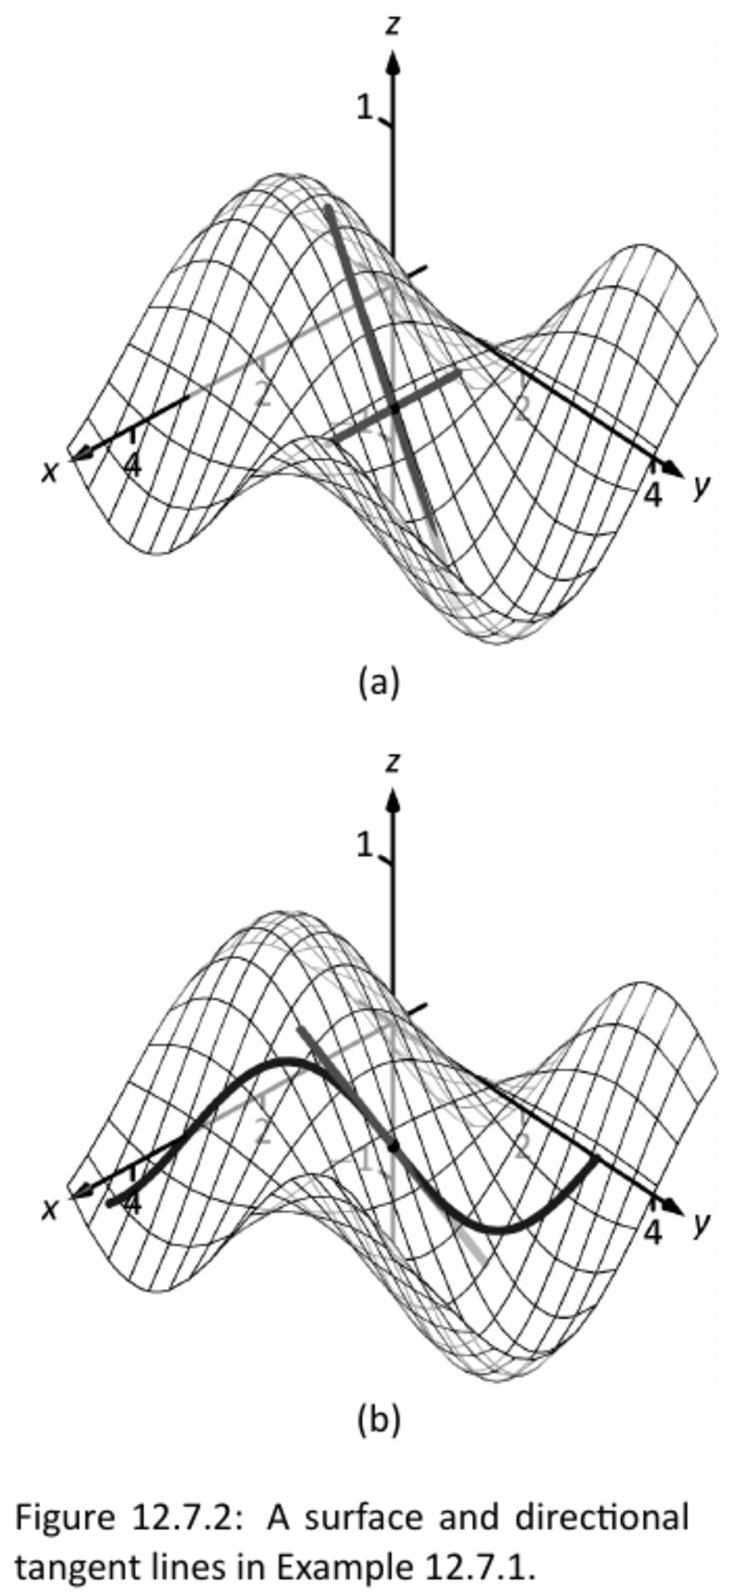
\includegraphics[height=8cm]{2022-2-C3/APEX_calculus_fig_12.7.2.pdf}


}}

\newpage

% «normal-e-gradiente»  (to ".normal-e-gradiente")
% (c3m222dpp 8 "normal-e-gradiente")
% (c3m222dpa   "normal-e-gradiente")
% (c3m222ptp 8 "retas-normais")
% (c3m222pta   "retas-normais")

%L normal1 = Numerozinhos.from(0, 0, 
%L     [[  .  .  .  .  .
%L         .  .  .  .  . 
%L         .  .  5  .  . 
%L         .  .  2  4  . 
%L         .  .  .  .  . ]])
%L normal1:topictu("12pt"):sa("normal1"):output()
%L normal2 = Numerozinhos.from(0, 0, 
%L     [[  .  .  .  .  .
%L         .  .  .  .  . 
%L         .  .  5  .  . 
%L         .  .  2  2  . 
%L         .  .  .  .  . ]])
%L normal2:topictu("12pt"):sa("normal2"):output()
%L normal3 = Numerozinhos.from(0, 0, 
%L     [[  .  .  .  .  .
%L         .  .  .  .  . 
%L         .  .  4  .  . 
%L         .  .  4  2  . 
%L         .  .  .  .  . ]])
%L normal3:topictu("12pt"):sa("normal3"):output()
\pu

\def\vecdx{{\vec{d}}_x}
\def\vecdy{{\vec{d}}_y}
\def\vecn {{\vec{n}}}
\def\nmat#1#2#3{\ensuremath{\pmat{#1 & \\ #2 & #3}}}

{\bf Vetores normais}

\scalebox{0.55}{\def\colwidth{9cm}\firstcol{

    Leia a seção sobre ``normal lines'' na p.741 do APEX Calculus (no
    capítulo 12 dele):

\ssk

{\scriptsize

% (find-books "__analysis/__analysis.el" "apex-calculus" "741" "Normal lines")
% (find-apexcalculuspage (+ 10 741)      "Normal lines")
%    http://angg.twu.net/2022.2-C3/APEX_Calculus_Version_4_cap_12.pdf#page=64
\url{http://angg.twu.net/2022.2-C3/APEX_Calculus_Version_4_cap_12.pdf\#page=64}

}

\ssk

Além das definições do livro nós vamos usar estas aqui. Sejam:
%
$$\begin{array}{rcl}
  A &=& (x_0,y_0,z_0) \\
  \vecn &=& \vecdx × \vecdy \\
  B &=& A + \vecdx \\
  C &=& A + \vecdy \\
  D &=& A + \vecn \\
  E &=& A - \vecn \\
  \end{array}
$$

% «exercicio-3»  (to ".exercicio-3")
% (c3m222dpp 8 "exercicio-3")
% (c3m222dpa   "exercicio-3")

{\bf Exercício 3.}

a) Digamos que $A=(2,1,2)$, $f_x=2$ e $f_y=3$. Então podemos
representar os pontos $A$, $B$ e $C$ como numerozinhos desta forma:

$$\ga{normal1}$$

Represente como numerozinhos os pontos $D$ e $E$.

}\anothercol{

Agora cada um dos diagramas de numerozinhos abaixo representa os
pontos $A$, $B$ e $C$ da construção acima, mas você é que vai ter que
descobrir quem são $x_0$, $y_0$, $z_0$, $f_x$, $f_y$, etc --
\ColorRed{e desenhar os pontos $D$ e $E$ em cada um dos casos}

\msk


Desenhe os pontos $D$ e $E$ nos diagramas de numerozinhos abaixo:

\msk

b) $\ga{normal2}$
\qquad
c) $\ga{normal3}$


}}





\newpage

% «exercicio-4»  (to ".exercicio-4")
% (c3m222dpp 9 "exercicio-4")
% (c3m222dpa   "exercicio-4")

{\bf Exercício 4.}

\scalebox{0.8}{\def\colwidth{8cm}\firstcol{

Este exercício é continuação do anterior.

\ssk

Agora vou passar a usar uma notação mais compacta ainda. Todas as
figurinhas abaixo representam diagramas de numerozinhos com
$(x_0,y_0)=(3,3)$, mas desenhados sem os eixos. Para cada uma delas
descubra quem são os pontos $D$ e $E$ da figura e desenhe os pontos
$A$, $B$, $C$, $D$ e $E$ num diagrama de numerozinhos de verdade.

\ssk

Às vezes você vai ter que desenhar dois
numerozinhos um em cima do outro.


}\anothercol{

\vspace*{0cm}

$\scalebox{0.7}{$
  \begin{array}{ccccc}
  \nmat 020 &
  \nmat 021 &
  \nmat 022 &
  \nmat 023 &
  \nmat 024 \\ \\
  \nmat 120 &
  \nmat 121 &
  \nmat 122 &
  \nmat 123 &
  \nmat 124 \\ \\
  \nmat 220 &
  \nmat 221 &
  \nmat 222 &
  \nmat 223 &
  \nmat 224 \\ \\
  \nmat 320 &
  \nmat 321 &
  \nmat 322 &
  \nmat 323 &
  \nmat 324 \\ \\
  \nmat 420 &
  \nmat 421 &
  \nmat 422 &
  \nmat 423 &
  \nmat 424 \\ \\
  \end{array}
  $}
$

}}


\newpage

{\bf Exercício 5.}


\scalebox{0.9}{\def\colwidth{12.5cm}\firstcol{

Este exercício é continuação do anterior.

\ssk

Leia a definição de gradiente na página 731
do

APEX Calculus (no capítulo 12):

\ssk

{\scriptsize

% (find-books "__analysis/__analysis.el" "apex-calculus" "741" "Normal lines")
% (find-apexcalculuspage (+ 10 731)      "Definition 12.6.2. Gradient")
% (find-apexcalculuspage (+ 10 741)      "Normal lines")
%    http://angg.twu.net/2022.2-C3/APEX_Calculus_Version_4_cap_12.pdf#page=54
\url{http://angg.twu.net/2022.2-C3/APEX_Calculus_Version_4_cap_12.pdf\#page=54}

}

\bsk

Acrescente a seguinte definição às que você usou nos exercícios 3 e 4,
%
$$G \; = A + \VEC{f_x, f_y, 0}
$$

e refaça todos os 25 itens do exercício 4 acrescentando o ponto $G$
neles.

\bsk

Daqui a pouco nós vamos ver qual é a relação desse vetor
$\VEC{f_x, f_y, 0}$ com o gradiente!...

}\anothercol{
}}




\newpage

{\bf Gradientes na prova}

% http://angg.twu.net/2022.2-C3/C3-quadros.pdf











%\printbibliography

\GenericWarning{Success:}{Success!!!}  % Used by `M-x cv'

\end{document}

%  ____  _             _         
% |  _ \(_)_   ___   _(_)_______ 
% | | | | \ \ / / | | | |_  / _ \
% | |_| | |\ V /| |_| | |/ /  __/
% |____// | \_/  \__,_|_/___\___|
%     |__/                       
%
% «djvuize»  (to ".djvuize")
% (find-LATEXgrep "grep --color -nH --null -e djvuize 2020-1*.tex")

 (eepitch-shell)
 (eepitch-kill)
 (eepitch-shell)
# (find-fline "~/2022.2-C3/")
# (find-fline "~/LATEX/2022-2-C3/")
# (find-fline "~/bin/djvuize")

cd /tmp/
for i in *.jpg; do echo f $(basename $i .jpg); done

f () { rm -v $1.pdf;  textcleaner -f 50 -o  5 $1.jpg $1.png; djvuize $1.pdf; xpdf $1.pdf }
f () { rm -v $1.pdf;  textcleaner -f 50 -o 10 $1.jpg $1.png; djvuize $1.pdf; xpdf $1.pdf }
f () { rm -v $1.pdf;  textcleaner -f 50 -o 20 $1.jpg $1.png; djvuize $1.pdf; xpdf $1.pdf }

f () { rm -fv $1.png $1.pdf; djvuize $1.pdf }
f () { rm -fv $1.png $1.pdf; djvuize WHITEBOARDOPTS="-m 1.0 -f 15" $1.pdf; xpdf $1.pdf }
f () { rm -fv $1.png $1.pdf; djvuize WHITEBOARDOPTS="-m 1.0 -f 30" $1.pdf; xpdf $1.pdf }
f () { rm -fv $1.png $1.pdf; djvuize WHITEBOARDOPTS="-m 1.0 -f 45" $1.pdf; xpdf $1.pdf }
f () { rm -fv $1.png $1.pdf; djvuize WHITEBOARDOPTS="-m 0.5" $1.pdf; xpdf $1.pdf }
f () { rm -fv $1.png $1.pdf; djvuize WHITEBOARDOPTS="-m 0.25" $1.pdf; xpdf $1.pdf }
f () { cp -fv $1.png $1.pdf       ~/2022.2-C3/
       cp -fv        $1.pdf ~/LATEX/2022-2-C3/
       cat <<%%%
% (find-latexscan-links "C3" "$1")
%%%
}

f 20201213_area_em_funcao_de_theta
f 20201213_area_em_funcao_de_x
f 20201213_area_fatias_pizza



%  __  __       _        
% |  \/  | __ _| | _____ 
% | |\/| |/ _` | |/ / _ \
% | |  | | (_| |   <  __/
% |_|  |_|\__,_|_|\_\___|
%                        
% <make>

 (eepitch-shell)
 (eepitch-kill)
 (eepitch-shell)
# (find-LATEXfile "2019planar-has-1.mk")
make -f 2019.mk STEM=2022-2-C3-derivadas-parciais veryclean
make -f 2019.mk STEM=2022-2-C3-derivadas-parciais pdf

% Local Variables:
% coding: utf-8-unix
% ee-tla: "c3dp"
% ee-tla: "c3m222dp"
% End:
